\chapter{Definición de una Arquitectura de Referencia para el Web Browser}
\label{chap5:ArqRefWB}


Para poder entender algún Browser se buscó en específico trabajos, papers, documentación gris a través de buscadores web como: IEEE Xplore, ACM digital Libray, Scopus y otros más, con tal de encontrar documentos formales sobre sus arquitecturas. Lo que más se encontró fueron blogs de desarrollo y White papers sobre Google Chrome, sin embargo llama la atención la escases en literatura sobre el tema. 


En vista a la poca, casi nula, documentación formal sobre el Navegador Web, la necesidad de hacer una Arquitectura de Referencia (AR) para entender cómo la arquitectura de este sistema puede relacionarse con el futuro desarrollo de otros sistemas, puede llegar a ser de gran utilidad para explicar los conceptos de seguridad detrás del Navegador. Se sabe que el Browser es un pieza de Software que ha sufrido varios cambios desde la década de los 90, por lo tanto entre los desarrolladores de esta herramienta ya existen convenciones de qué elementos funcionan mejor. Por consiguiente, no es de extrañar que diferentes browsers estén construidos de formas muy similares, y puedan ser conceptualizados en una AR que manifieste los componentes, mecanismos de comunicación y funciones de esta pieza de Software. 


La AR a construir en este trabajo, fue realizada principalmente a través de la abstracción de las propuestas actuales de los Web Browsers más usados: Google Chrome, Internet Explorer y Firefox (propuesta Electrolysis). Primero se identificarán y analizarán los stakeholders, se identificarán los casos de uso relacionados a cada uno de estos stakeholders y se dará una descripción breve. Luego se presentan 2 patrones que formarán parte de nuestra AR; Browser Infrastructure Pattern donde están los componentes principales, la comunicación con el host y la interacción entre éstos. Y luego el patrón RendererContentTab que muestra el interior del encargado de renderizar una página web. Éstos patrones serán descritos utilizando un template POSA \cite{buschman1996system} y notación UML para precisar cómo en una AR se relaciona los componentes. 

\section{Casos de Uso del Browser}
	\subsection{Stakeholders (actores) y Concerns de estos}
	Se es necesario encontrar los actores (definido por sus roles) que participan en el uso y operación del Navegador, éstos son:
		\subsubsection{Browser User (BU)}
		De este stakeholder depende que se realice el inicio de una petición para buscar una página web, recurso o servicio (Sin éste la utilidad del Web Browser es nula). Una entidad no humana, como un plugin, extensión o instancia de una página web, pueden requerir hacer peticiones por medio de las interfaces del navegador, con la intención de cumplir con el deseo del usuario del host de mostrar el contenido en el Browser.
		\subsubsection{Host (H)}
		Para este caso nos referiremos solamente a la máquina cliente dónde se aloja el Web Browser. Ésta crea los procesos necesarios para iniciar el Navegador, además de entregar un ambiente al Browser para que éste pueda funcionar adecuadamente.  Esta identidad se encarga de aplicar políticas de seguridad sobre el Browser cuando se necesiten realizar operaciones o el navegador desee crear nuevos procesos.
		\subsubsection{Provider (P)}
		Es toda la infraestructura relacionada con el Servicio Web que pudiera entregar una máquina remota a un Navegador. Este puede ser un: Web Server, Web Aplicación, Servicio de actualización del Browser, etc. Su interacción con el Browser se limita a entregar contenido a éste.
		\subsection{Casos de Uso}
Los casos de usos y actores están listados a continuación. Notar que se presentarán aquellos casos de uso relacionados exclusivamente con el Browser.

\subsubsection{Casos de Uso para Browser User (BU)}
		El BU representa todas las interacciones posibles del usuario con el Browser y sin él no habría razón para la existencia del navegador; un servidor tampoco existiría dado el mismo principio. Al encontrar los casos de uso de este stakeholder veremos las preocupaciones de éste, lo que nos permitirá entender las necesidades de seguridad para proteger al navegador. Los casos de uso principales de éste son: Realizar Request, Cancelar Request y Guardar Recurso.
			\begin{enumerate}	
				\item Realizar Petición/Request: El caso de uso más importante de este sistema, se basa en la arquitectura cliente/servidor. Esta acción considera la petición de recursos al Provider (P) y la búsqueda del recurso bajo la URI dada y la consecuente respuesta de éste. La descarga no es siempre necesaria, pues existe lo que se conoce como una petición \textit{preflight} donde solo se envía una petición para saber si es seguro realizar una petición/\textit{request}. Tanto petición como respuesta se han condensado en un solo caso de uso. Este caso de uso considera la visualización del recurso en el Host a través del periférico predeterminado.
				\item Cancelar request: Un BU pide al Browser detener la búsqueda y todo proceso en tránsito. Si el recurso es obtenido por el Browser, la detención de éste puede considerar la detención del componente Renderer para mostrar por pantalla la proyección de la página web obtenida.			
				\item Guardar recurso: Un BU puede necesitar guardar el recurso recientemente adquirido en el sistema de archivos del host (H). El caso de uso inicia una vez que el BU haya manifestado dónde desea guardar el recurso.
			\end{enumerate}

\subsubsection{Casos de Uso para el Host (H)}
Los casos de uso del Host representan todas las interacciones que relacionan servicios provistos al BU al hacer uso de \textit{system calls}, por medio del Browser. El Host debe para esto contar con la respuesta explícita del usuario detrás de BU. Los casos de uso principales de H son: Operación CRUD en el sistema de archivos del host, Monitorear proceso y Pedir recursos.
			\begin{enumerate}
				\item Operación CRUD en el sistema de archivos del host: Acción realizada cuando el Browser obtiene una solicitud explícita o no (automática), del usuario para realizar acciones que involucren permitir el acceso al sistema de archivos para: leer, escribir o modificar/eliminar algún recurso del host.

				\item Monitorear proceso: En un browser es normal la comunicación entre los procesos que lo componen y el Sistema Operativo por medio de un canal de comunicación, en especial cuando se necesita ver la cantidad de recursos usados.

				\item Pedir recursos: Bajo el pedido explícito del usuario, la entidad BU, se requieren recursos para iniciar las operaciones deseadas. Estos recursos son obtenidos a partir de llamadas al sistema al host.
			\end{enumerate}

		\subsubsection{Casos de Uso para el Proveedor (P)}
		La meta del Proveedor es escuchar las peticiones provenientes de diversos tipos de BU que necesiten los servicios o recursos del Proveedor. En este escenario tan heterogéneo y distribuido que es la Internet, se enfocará solamente en las peticiones de BU. Además, no para toda \textit{request} del BU habrá un \textit{response} de P, pues puede pasar que BU esté solamente intentando averiguar si P existe.
			\begin{enumerate}
				\item Escuchar requests: P siempre está escuchando en sus puertos habilitados a posibles peticiones de sus clientes. Una petición es recibida en un formato que P pueda interpretar y en consecuencia realizar las acciones correspondientes que BU le pide. 
				\item Enviar Response: Por cada solicitud del cliente, en este caso el Web Browser, habrá una respuesta/response por parte del P con la data Resource asociada. Este caso de uso no se realiza, si dentro del header de uno de los paquetes está indicado que la petición fue hecha en modo \textit{preflight}.
				\item Crear recurso: Por cada recurso que P crea, una URL única será usada para ser identificada en la Internet. Un BU hace uso de tal URL para adquirir el recurso, mientras el host del Proveedor lo deje visible.
				\item Configurar opciones: definir distintas medidas en el Proveedor como: acceso a recursos, acceso de Browser users, etc.
			\end{enumerate}

		Los casos de Uso descritos anteriormente se pueden divisar en la Figura \ref{fig:CUBrowser}

	    \begin{figure}[h!t]
	        \centering
	        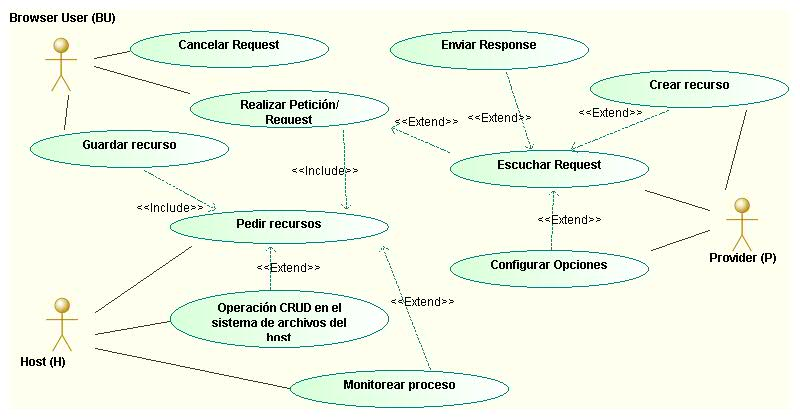
\includegraphics[scale=0.45]{figures/chap4/UCBrowser.jpg}
	        \caption{Diagrama de Caso de Uso del Web Browser.}
	        \label{fig:CUBrowser}
	    \end{figure}


\section{Patrón Browser Infrastructure}
\label{chap4:BrokerPatt}
\subsection{Intent}
El patron Browser Infrastructure pattern permite la realización de la solicitud o \textit{request} de un recurso web en la Internet por parte de un BU, que es un usuario del Host que utiliza un navegador. El patrón permite visualizar la comunicación entre los componentes que conforman el browser así como la comunicación con el proveedor, al que se le realiza el \textit{request}.

\subsection{Ejemplo}
Dentro de un host es posible que exista una falta de recursos que necesite el usuario que lo opera. La solicitud de servicios o recursos externos es una de las razones de existir de la Internet. Esta operación es posible de realizarla de diferentes maneras, todo depende de lo que el Provider desea entregar.

\subsection{Contexto}
Browser User se encuentra al interior del Host y el Provider es accedido a través de Internet.  Es común que el contacto se da a través de aplicaciones web, servers que se comunican a través del protocolo HTTP. Para poder visualizar los recursos que el usuario del host puede necesitar y que el proveedor pueda quizás entregar, un navegador web permite completar tal labor de forma transparente al usuario.
\subsection{Problema}
Algunos usuario del Host puede que necesiten obtener recursos desde un Provider, pero el usuario puede que necesite utilizarlos en algún formato en especial o que sean presentados por pantalla para ser mejor visualizados. En este caso, si no se utiliza la herramienta adecuada puede que no sirva de mucho haber conseguido el recurso si no se puede ocupar correctamente. ¿Cómo pueden el Host y Provider estar preparados para esta situación?
La solución a este problema debe resolver las siguientes problemáticas:
\begin{itemize}
	\item Transparencia: el usuario detrás del Host no se debe preocupar de la maquinaria que existe mientras se realiza una petición a un Provider.
	\item Estabilidad/Aislación: cada \textit{request} realizada no debe interferir con las otras.
	\item Heterogeneidad: Sin importar el tipo de Provider con el que se comunique, el Browser User debe poder comunicarse con cualquier tipo de Provider y también debe poder mostrar adecuadamente al usuario el recurso obtenido.
	\item Disponibilidad: El usuario del Host debe ser capaz de poder realizar peticiones en todo momento, sin perder fluidez.
\end{itemize}

\subsection{Solución}
Un Web Browser puede satisfacer las \textit{request} del user del Host a través de un Browser User, ya sea por una o varias instancias de Browser User, lo que permite tener una diversidad de opciones para navegar por sitios de Internet. Un Browser debe ser capaz de poder entregar una navegación rápida y estable, sin que cada sitio accedido afecte a los otros recursos adquiridos.
\subsection{Estructura}
El Browser Client (BC) es la entidad que representa el proceso principal de un Navegador Web y comprende la cantidad mínima de componentes que constituye un Web Browser. Browser Client, Sandbox, GPU Instance (GPUI) y Plugin son del tipo Process (Pr), que residen dentro de un Host (H) con un cierto tipo de sistema Operativo (OS). La mayoría de los navegadores existentes usan un componente central para realizar las operaciones que necesitan afectar al Host del Browser. La figura \ref{fig:BIPatt} muestra el diagrama del clases para el patrón Browser Infrastructure. Por cada recurso que un BC solicite, se crearán Sandbox (S) que alojarán una instancia del patrón RendererContentTab el que permiten realizar la navegación y posterior visualización del recurso.
El componente BC actúa como un broker de las solicitudes de las Sandbox, lo que permite tener un control fino de los mensajes enviados, usando IPC/IPDL/COM, entre los procesos que se comunican. El GPU Instance y Plugins son elementos que pueden comunicarse directamente con el Sandbox, de esta manera cualquier necesidad de recursos del Host pasarán también por el Browser Client. 
Un usuario que desee hacer un \textit{request} de un recurso en Internet por medio de un navegador es lo que llamaremos Browser User (BU). Éste usa el Browser Client para realizar peticiones al Provider, donde éste último posiblemente utilice un Web Server para ese cometido (Figura \ref{fig:BIPatt})

	    \begin{figure}[h!t]
	        \centering
	        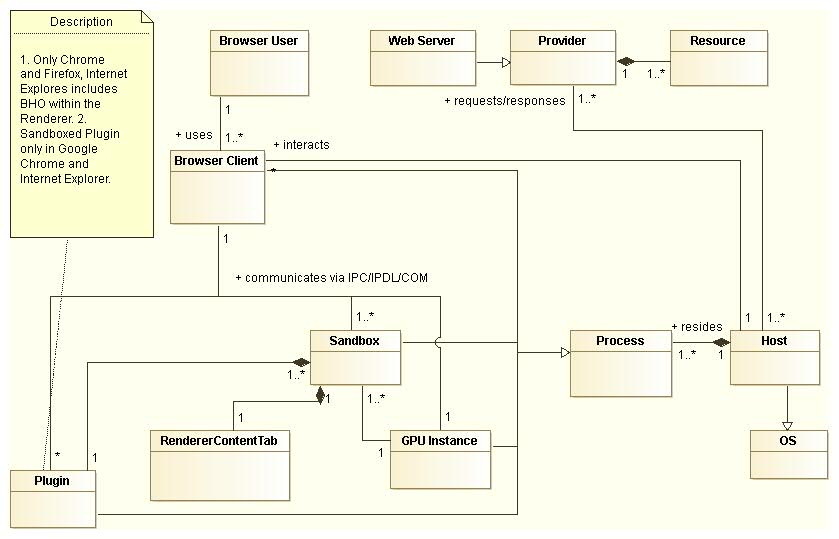
\includegraphics[scale=0.45]{figures/chap4/browserInfraPattern.jpg}
	        \caption{Componentes de alto nivel del Browser.}
	        \label{fig:BIPatt}
	    \end{figure}

\subsection{Dinámica}
Los casos de uso relacionados al patrón son los siguientes:
\begin{itemize}
	\item Realizar request (actor: Browser User)
	\item Cancelar request (actor: Browser User)
	\item Guardar recurso (actor: Browser User)
	\item Recibir Request (actor: Provider)
	\item Pedir recursos (actor: Host)
\end{itemize}
Detallaremos el caso de uso Realizar Request (Figura \ref{fig:SecReq}):
\subsubsection{Sumario} Un Browser User requiere de abrir un recurso URL que puede ser obtenido mediante el uso del protocolo HTTP, según los requerimientos del Provider. El Browser Client será usado por un Browser User para poder realizar la visualización del recurso URL.
\subsubsection{Actor} Browser User
\subsubsection{Precondiciones} El Host debe tener uno o más Browser Client para el usuario del Host. Además de estar conectado a una red o Internet. El Provider al que se desea contactar también debe estar disponible.
\subsubsection{Descripción}
Nota: Los mensajes entre el Browser Client y el Sandbox pueden ser tanto síncronos como asíncronos. No especificaremos en gran detalle , pues lo que importa en este trabajo será el origen y destino de los mensajes (no está dentro del ámbito ver la sincronización).
	\begin{enumerate}
		\item Un Browser User requiere acceder a una URL para obtener cierto recurso de un Provider, para esto usa un Browser Client ya instanciado por el Host. En el interior del Sandbox, existe una instancia del patrón RendererContentTab en su interior. 
\item El Sandbox requiere los recursos del Host para obtener lo que hay detrás de la URL. Una petición es realizada desde el Sandbox al Browser Client a través de un canal de comunicación como: IPC, IPDL o COM (dependiendo el tipo de Browser usado), usando la API limitada que posee para comunicarse a un proceso de mayor privilegio. 
\item El Browser Client recibe la solicitud, verifica a través de su motor de políticas/normas si la acción del Sandbox puede ser permitida.
\item Si es permita la acción del Sandbox, se utilizará la Network API que contiene el Browser Client para obtener recursos del Host (a través de llamadas al sistema). El Browser Client se comunica internamente con el Host, y este último debe revisar sus políticas y asegurarse que el Browser Client posee el privilegio de hacer la petición del recurso del Host.
\item Si se permite el acceso el recurso, el Browser Client podrá realizar un \textit{request} a través de la Network API. Si el \textit{request} no es del tipo \textit{pre-flight}, el Provider recibirá el \textit{request} y trabajará sobre la petición.
\item El Provider enviará un response al \textit{request} enviado. Dependiendo como esté implementado el Browser Client, este podría o no tener que esperar a la respuesta (síncrono o asíncrono) del Provider.
\item Una vez obtenida la respuesta esta es almacenada en cache o podría ser guardada dentro del Host. 
\item La respuesta del \textit{request} es enviada por el canal de comunicación al Sandbox del que se originó y posteriormente al RendererContentTab. Si fue recibida una respuesta por parte de la \textit{request}, el RendererContentTab está listo para preparar el parsing de la página web o utiliza un plugin o GPU para apoyar la visualización del recurso obtenido por la URL. En caso contrario el RendererContentTab dentro del Sandbox creará una página de error.
	\end{enumerate}
\subsubsection{Curso Alternativo} 
\begin{itemize}
\item El Provider no esté disponible.
\item El recurso al que apunta la URL no exista.
\item Se cancela el \textit{request} realizado.
	\end{itemize}
\subsubsection{Condiciones póstumas} El Browser recibe el recurso indicado por la URL y se muestra por el perísférico la salida del recurso al usuario del Host.
	    \begin{figure}[h!t]
	        \centering
	        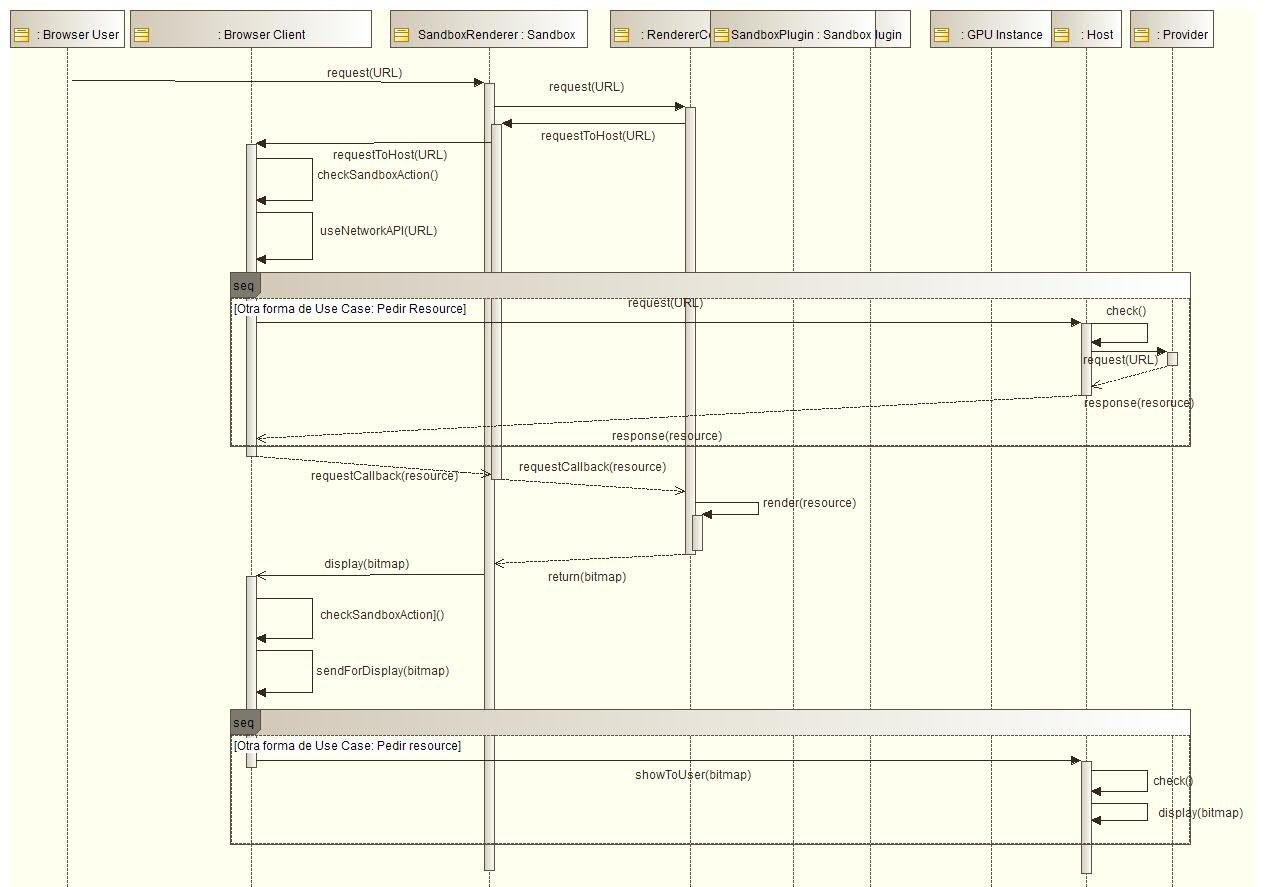
\includegraphics[scale=0.35]{figures/chap4/requestResource.jpg}
	        \caption{Diagrama de Secuencia: Browser User Realiza request.}
	        \label{fig:SecReq}
	    \end{figure}
\subsection{Implementación}
\begin{itemize}
\item El Sandbox puede ser implementado de diversas maneras. Google Chrome [referencia a página de sandbox de cg] se basa en no reinventar la rueda y utiliza los mecanismos de protección que Windows ya tiene incorporados para proteger al usuario, evitando que el proceso no tenga acceso al sistema de archivos y teniendo una API de llamadas al sistema muy restrictivas en el RendererContentTab. Google Chrome, Firefox e Internet Explorer asumen que los Sandoboxs son procesos que deben regirse bajo el principio de menor privilegio (least privilege). La mínima configuración del Sandbox se compone de 2 procesos: El proceso privilegiado o Broker que es representado por el BrowserClient, y el o los procesos que están bajo el Sandbox o targets.
\item Para hacer cumplir con el Same Origin Policy Google Chrome, Firefox e Internet Explorer utilizan diferentes esquemas, por ejemplo: Google Chrome deja el trabajo a su Renderer (RendererContentTab en este caso) para dejar aisladas las páginas/recursos de diversos sitios.
\end{itemize}
\subsection{Consecuencias}
El patrón Browser Infrastructure provee los siguientes beneficios:
\begin{itemize}
	\item Transparencia: La navegación del usuario se realizará casi de manera automática, solo en casos muy puntuales el usuario tendrá que tomar una decisión sobre el recurso que desea pedir.
\item Estabilidad/Aislación: Gracias a que el Browser Client, Sandbox, Plugin y GPU Instance son procesos del Host independientes, el fallo de uno no generará problemas en el otro (crash, corrupción de memoria, etc).
	\item Heterogeneidad: Dado que cada Browser Client trata de seguir los estándares de la W3C, toda página que también siga éstas guías podrá ser visualizada, así como también otro tipo de recursos.
	\item Disponibilidad: Cada proceso es independiente y posee sus propias hebras de ejecución, y fueron creadas específicamente para que la interfaz de usuaria pueda mantenerse fluida para el usuario.
\end{itemize}
Al mismo tiempo el patrón posee las siguientes debilidades:
\begin{itemize}
	\item Dado que se inician procesos independientes para navegar a un recurso (dependiendo el esquema que utilice el browser), es posible que una gran cantidad de recursos se vayan a usar para mantener todo abierto.
	\item Aquellos Provider que no hayan cumplido con las especificaciones de la W3C, mostraran su resource de forma incorrecta por el Web Browser.
\end{itemize}
\subsection{Ejemplo Resuelto}
Con el patrón entregado ahora es posible poder navegar de forma fluida a todos los recursos en la Internet que deseamos. Es posible proveer a través de la aislación de los componentes: rapidez, seguridad y estabilidad. El Browser User solamente se molestará en la navegación, cuando se requiera de su autorización para ingresar a ciertos recursos del Host que sean privilegiados, como el sistema de archivos. Cada usuario del Host, puede utilizar el Browser Client que desee, dado que cada uno de ellos es aislado por procesos independientes, así también los otros Browser Clients entre si.

\subsection{Usos Comúnes}
\begin{itemize}
	\item Google Chrome
	\item Internet Explorer
	\item Firefox
\end{itemize}
\subsection{Patrones Asociados}
\begin{itemize}
	\item Reference Monitor [Fer13]
	\item Policy authorization
\end{itemize}
